%%
%% This is file `tikzposter-template.tex',
%% generated with the docstrip utility.
%%
%% The original source files were:
%%
%% tikzposter.dtx  (with options: `tikzposter-template.tex')
%%
%% This is a generated file.
%%
%% Copyright (C) 2014 by Pascal Richter, Elena Botoeva, Richard Barnard, and Dirk Surmann
%%
%% This file may be distributed and/or modified under the
%% conditions of the LaTeX Project Public License, either
%% version 2.0 of this license or (at your option) any later
%% version. The latest version of this license is in:
%%
%% http://www.latex-project.org/lppl.txt
%%
%% and version 2.0 or later is part of all distributions of
%% LaTeX version 2013/12/01 or later.
%%


\documentclass{tikzposter} %Options for format can be included here

\usepackage{todonotes}

\usepackage[tikz]{bclogo}
\usepackage{lipsum}
\usepackage{amsmath}

\usepackage{booktabs}
\usepackage{longtable}
\usepackage[absolute]{textpos}
\usepackage[it]{subfigure}
\usepackage{graphicx}
\usepackage{cmbright}
%\usepackage[default]{cantarell}
%\usepackage{avant}
%\usepackage[math]{iwona}
\usepackage[math]{kurier}
\usepackage[T1]{fontenc}


%% add your packages here
\usepackage{hyperref}
% for random text
\usepackage{lipsum}
\usepackage[english]{babel}
\usepackage[pangram]{blindtext}

\colorlet{backgroundcolor}{blue!10}

 % Title, Author, Institute
\title{New York City Taxi Trip Duration}
\author{Qin Zhang$^1$}
\institute{$^1$ Chongqing Technology and Business University, China 
}
%\titlegraphic{logos/tulip-logo.eps}

%Choose Layout
\usetheme{Wave}

%\definebackgroundstyle{samplebackgroundstyle}{
%\draw[inner sep=0pt, line width=0pt, color=red, fill=backgroundcolor!30!black]
%(bottomleft) rectangle (topright);
%}
%
%\colorlet{backgroundcolor}{blue!10}

\begin{document}


\colorlet{blocktitlebgcolor}{blue!23}

 % Title block with title, author, logo, etc.
\maketitle

\begin{columns}
 % FIRST column
\column{0.5}% Width set relative to text width

%%%%%%%%%% -------------------------------------------------------------------- %%%%%%%%%%
 %\block{Main Objectives}{
%  	      	\begin{enumerate}
%  	      	\item Formalise research problem by extending \emph{outlying aspects mining}
%  	      	\item Proposed \emph{GOAM} algorithm is to solve research problem
%  	      	\item Utilise pruning strategies to reduce time complexity
%  	      	\end{enumerate}
%%  	      \end{minipage}
%}
%%%%%%%%%% -------------------------------------------------------------------- %%%%%%%%%%


%%%%%%%%%% -------------------------------------------------------------------- %%%%%%%%%%
\block{Introduction}{

The competition dataset is based on the 2016 NYC Yellow Cab trip record data made available in Big Query on Google Cloud Platform. The data was originally published by the \emph{NYC Taxi} and Limousine Commission (TLC). The data was sampled and cleaned for the purposes of this playground competition. Based on individual trip attributes, participants should predict the duration of each trip in the test set.

The project provided 1458644 pieces of effective data for the construction of machine learning model. The purpose of the project is to predict the trip-duration time of passengers through "characteristics" such as pickup-datetime and dropoff-datetime.	

}
%%%%%%%%%% -------------------------------------------------------------------- %%%%%%%%%%


%%%%%%%%%% -------------------------------------------------------------------- %%%%%%%%%%
\block{Data Description}{
\begin{itemize}
    \item
    %\emph{Group Outlying Aspects Mining}
    The data set has a total of \emph{1458644 lines and 10 features}, which is a regression item.

    \item
    \emph{10 features}: ID, Vendor-id, Pickup-datetime, Dropoff-datetime, Passenger-count, Pickup-longitude, Pickup-latitude, Dropoff-longitude, Dropoff-latitude, Store-and-fwd-flag.

     \item
    \emph{Trip-duration}: Duration of the trip in seconds.
    
\end{itemize}

\begin{tikzfigure}%[Overall architecture of \emph{GOAM} algorithm]
%  \includegraphics[width=0.8\linewidth]{figures//framework.pdf}
    %\missingfigure[figcolor=white]{Testing figcolor}
    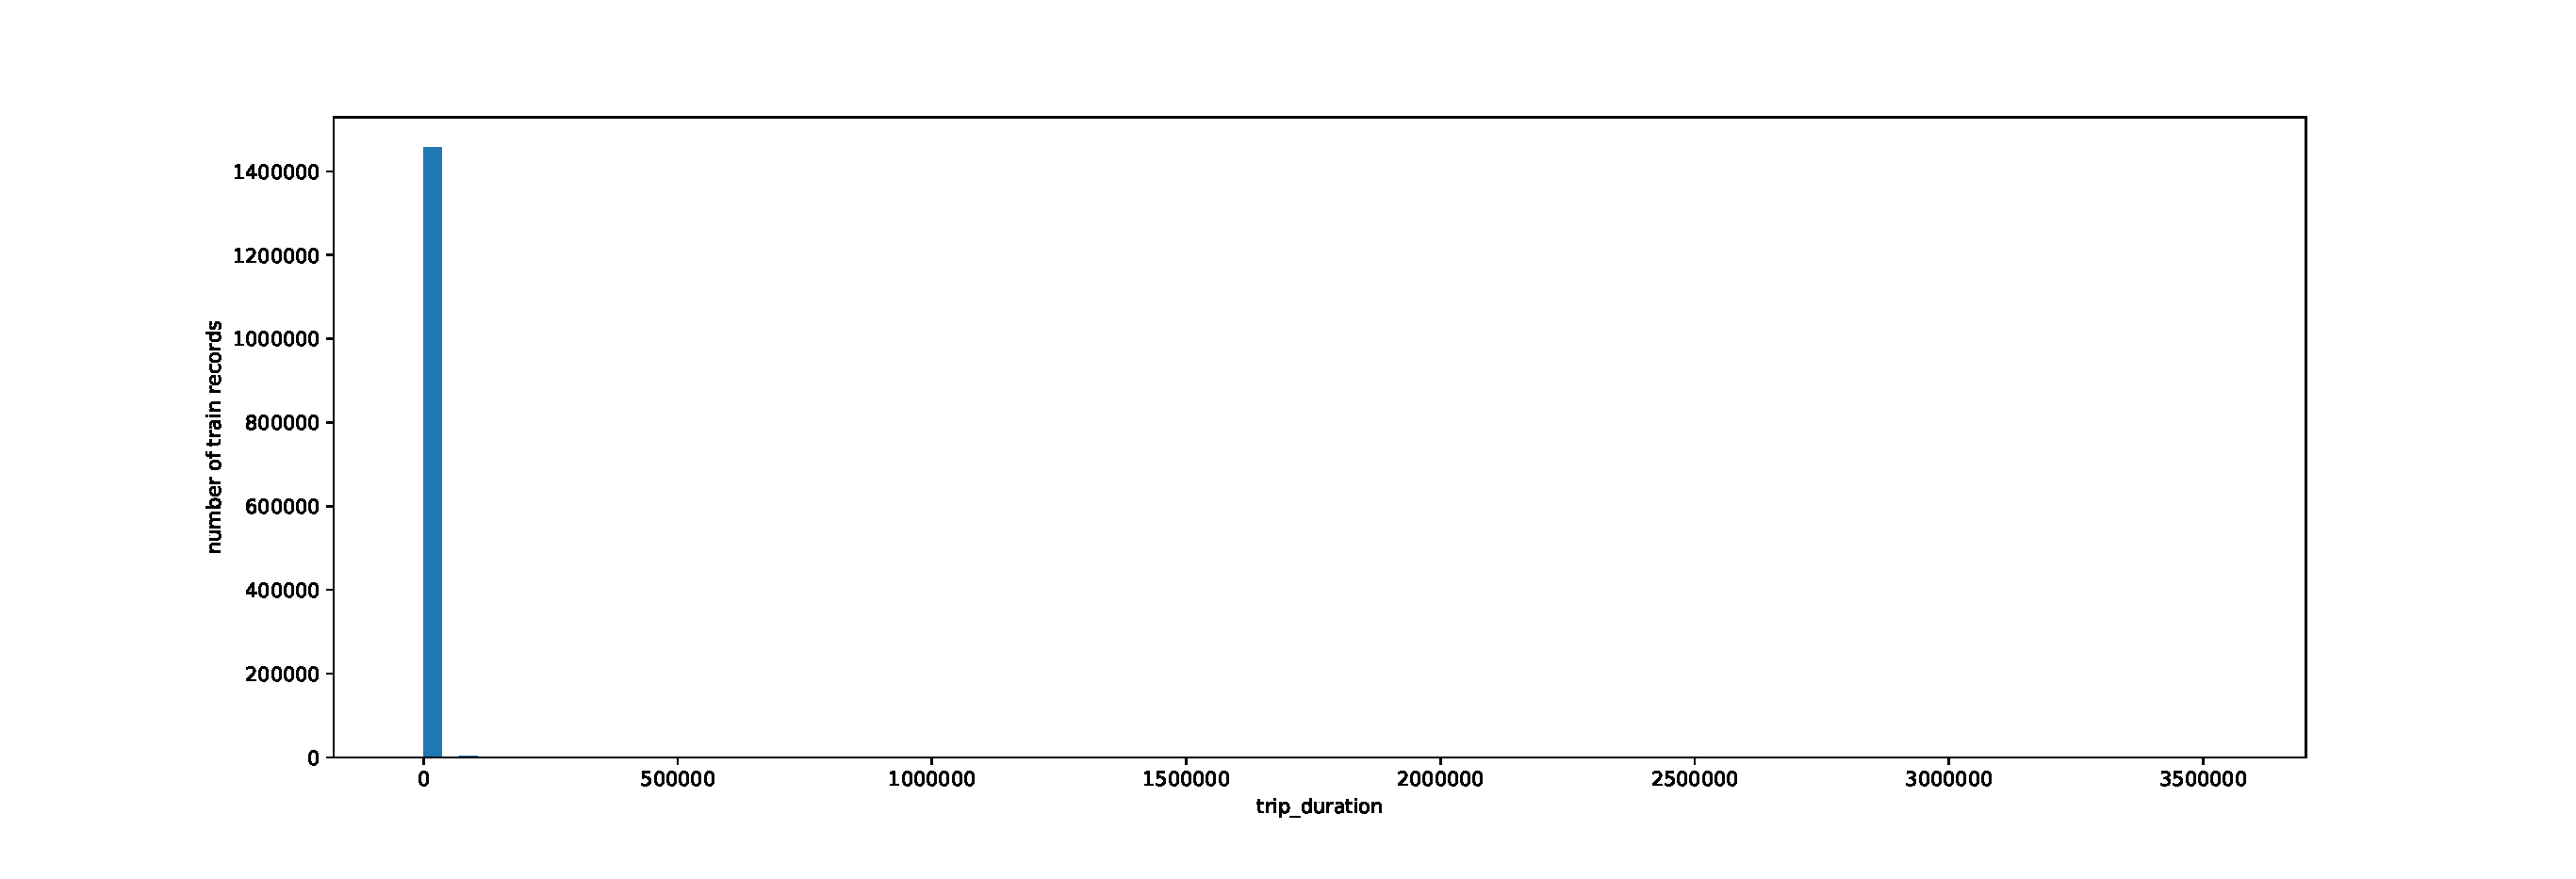
\includegraphics[width=0.3\textwidth]{figure//fig-1.eps}\\
\end{tikzfigure}

}
%%%%%%%%%% -------------------------------------------------------------------- %%%%%%%%%%


%%%%%%%%%% -------------------------------------------------------------------- %%%%%%%%%%

%\note{Note with default behavior}

%\note[targetoffsetx=12cm, targetoffsety=-1cm, angle=20, rotate=25]
%{Note \\ offset and rotated}

 % First column - second block


%%%%%%%%%% -------------------------------------------------------------------- %%%%%%%%%%
\block{Feature Engineering}{
  		
\begin{description}
  	\item[Outlier Processing]
   \end{description}

 \begin{itemize}
    \item  
  According to the relationship between longitude and latitude position and travel duration, abnormal data can be filtered out. Therefore, according to the analysis, the interference data within 1 million will be deleted. Selecting appropriate time data will help to train the model and improve the experimental accuracy.
   \item
  \emph{Passenger-count} is the number of passengers in the vehicle. According to the analysis of Fig. 2, the number of passengers varies from 0 to 9. Therefore, we need to delete the data with 0 passengers.
 
  \end{itemize}
  
\begin{description}
   \item[Feature Processing]
   \end{description}
   
 \begin{itemize}
    \item  
   Store-and-fwd-flag indicates whether the trip record was held in vehicle memory before sending to the vendor because the vehicle did not have a connection to the server. Y=store and forward, N=not a store and forward trip. We convert its character identification into numbers for easy analysis.
    \item 
   Add month, week and day. From the perspective of the trend, the overall taxi time has been increasing from January to June 2016. It may be that users are gradually accustomed to taking a taxi from a longer distance, or it may be that more and more vehicles are driving on the road or the weather is bad, causing traffic congestion. In this article, the original pickup-datetime is divided into hour, day of week and month.
    \item 
   Create a distance feature. According to the longitude and latitude in the known data, the distance between the starting position and the ending position of the taxi is calculated according to the formula.
   \end{itemize}
\begin{description}
   \item[Feature Visualization]
   \end{description}
   \begin{itemize}
    \item 
   Deleting invalid features can improve the experimental effect. The following is a visualization of three randomly selected features:
   \end{itemize}
   
%    \item
%    The histogram of $G_q$ on three features are as follows.


\begin{center}
    \begin{minipage}{0.3\linewidth}
    \centering
    \begin{tikzfigure}
    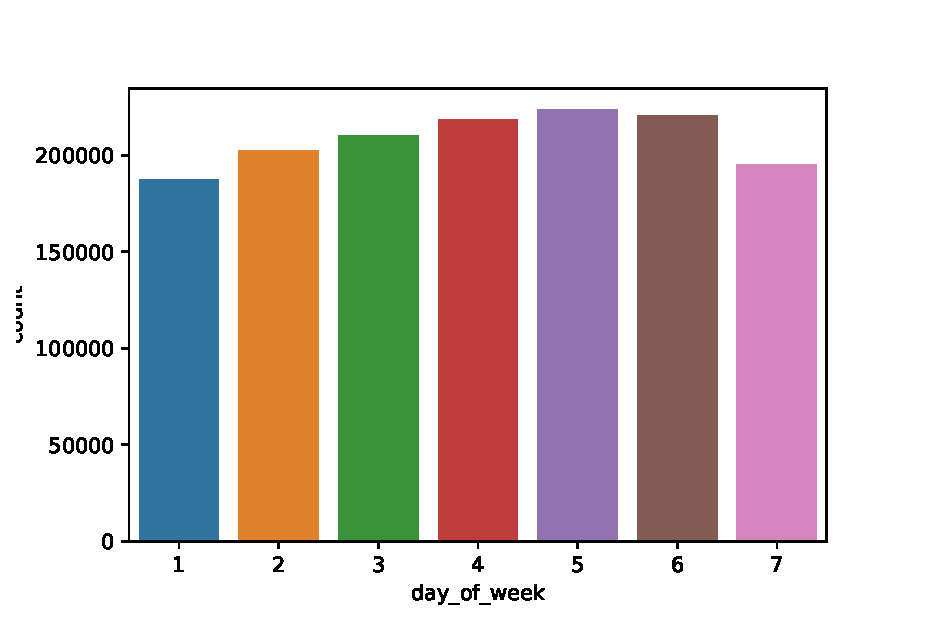
\includegraphics[width=0.8\textwidth]{figure//fig-8.eps}\\
    %\missingfigure[figcolor=white]{Testing figcolor}
    {\small{day_of_week}}
    \end{tikzfigure}%
    \end{minipage}
    \hfill
    \begin{minipage}{0.3\linewidth}
    \centering
    \begin{tikzfigure}
    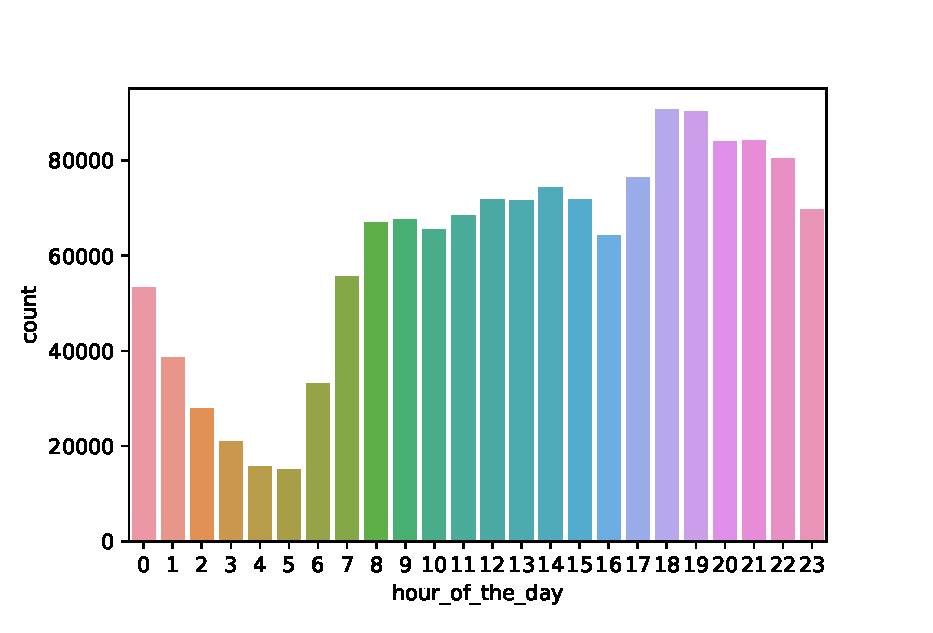
\includegraphics[width=0.8\textwidth]{figure//fig-9.eps}\\
    %\missingfigure[figcolor=white]{Testing figcolor}
    {\small{hour_of_the_day}}
    \end{tikzfigure}%
    \end{minipage}
    \hfill
    \begin{minipage}{0.3\linewidth}
    \centering
    \begin{tikzfigure}
    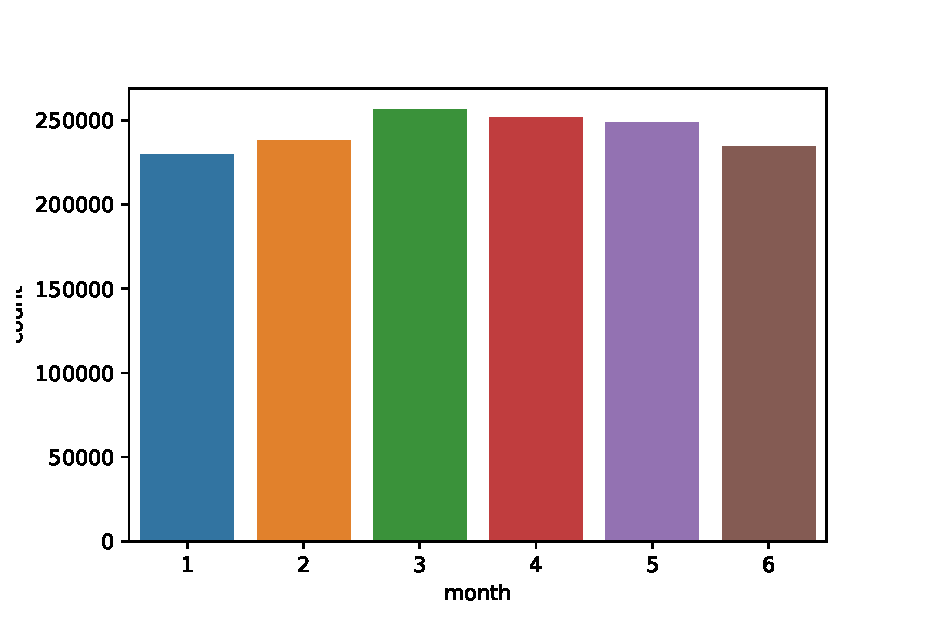
\includegraphics[width=0.8\textwidth]{figure//fig-10.eps}\\
    %\missingfigure[figcolor=white]{Testing figcolor}
    {\small{month}}
    \end{tikzfigure}%
    \end{minipage}
\end{center}

}
%%%%%%%%%% -------------------------------------------------------------------- %%%%%%%%%%


% SECOND column
\column{0.5}
 %Second column with first block's top edge aligned with with previous column's top.


%%%%%%%%%% -------------------------------------------------------------------- %%%%%%%%%%
\block{Feature Engineering}{
  		

\begin{description}
\item[Feature filtering]
\end{description}
\begin{itemize}
    \item 
Through the analysis of feature related data and heat map, the relationship between features can be obtained. It can be seen from the figure that the selected features are important.
\end{itemize}

   

\begin{tikzfigure}%[Overall architecture of \emph{GOAM} algorithm]
%  \includegraphics[width=0.8\linewidth]{figures//framework.pdf}
    %\missingfigure[figcolor=white]{Testing figcolor}
    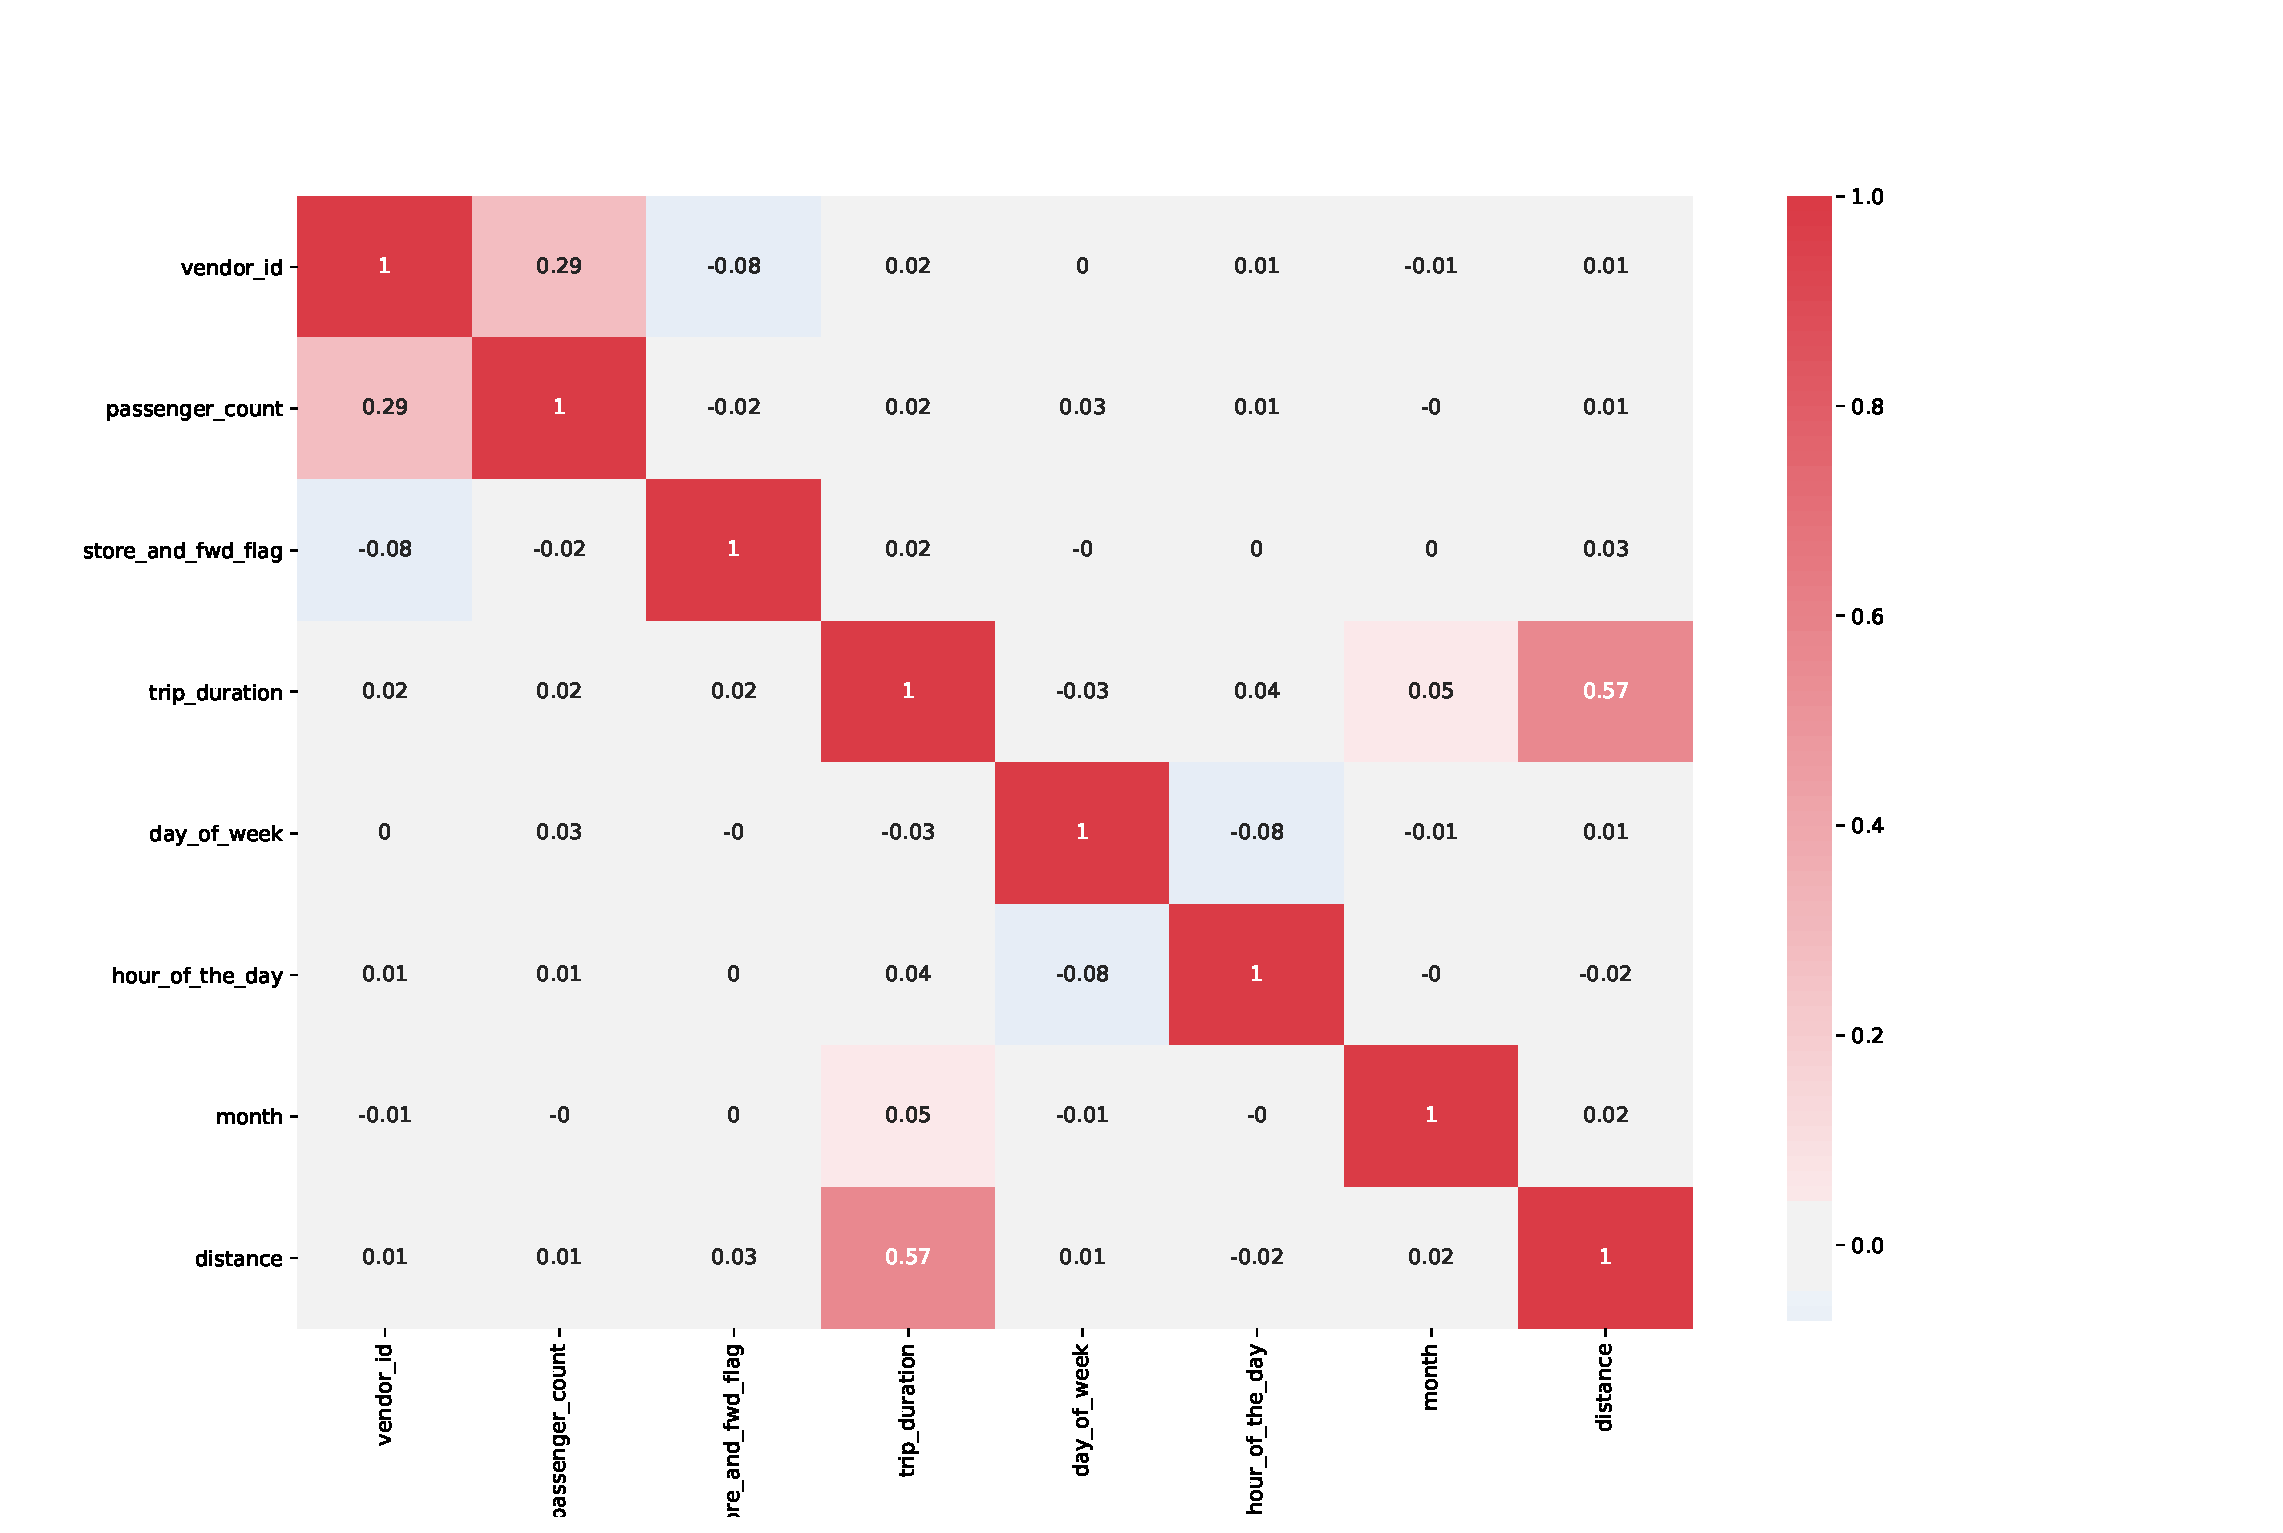
\includegraphics[width=0.3\textwidth]{figure//fig-6.eps}\\
\end{tikzfigure}
}
%%%%%%%%%% -------------------------------------------------------------------- %%%%%%%%%%

%%%%%%%%%% -------------------------------------------------------------------- %%%%%%%%%%
\block[titleleft]{Experiment}
{
\begin{description}
   \item[Model Introduction]
   \end{description}

   \begin{itemize}
    \item 
    Three models were selected in this experiment: LGBMRegressor, LinearRegression and DecisionTreeRegressor. 
    \item 
    The division ratio of training set and test set is set to 0.3.
   \end{itemize}

\begin{description}
     
    \item[Evaluation Indicator]
\end{description}

\begin{itemize}
 \item
${MSE = \frac{1}{m}{\sum\limits_{i = 1}^m {\left( {f\left( {{x_i}} \right) - {y_i}} \right)} ^2}}$

\item
${MAE = \frac{1}{N}\sum\limits_{i = 1}^N {\left| {{y_i} - f\left( {{x_i}} \right)} \right|} }$

\item
${RMSE = \sqrt {\frac{1}{N}\sum\limits_{i = 1}^N {{{\left( {{y_i} - f\left( {{x_i}} \right)} \right)}^2}} } }$

    
\end{itemize}

\begin{description}
     
    \item[Experimental Result]
\end{description}

\vspace{.5cm}



\begin{tabular}{c|c|c|c}
 \toprule
\textbf{Model} & \textbf{LGBMRegressor}      & \textbf{LinearRegression} & \textbf{DecisionTreeRegressor} \\
\midrule
R2\_score      & 0.66                        & 0.35                      & 0.3                            \\
MSE            & {\color[HTML]{FE0000} 0.22} & 0.42                      & 0.45                           \\
MAE            & {\color[HTML]{FE0000} 0.32} & 0.46                      & 0.46                           \\
RMSE           & {\color[HTML]{FE0000} 0.47} & 0.65                      & 0.67  \\
 \bottomrule
\end{tabular}


\vspace{.8cm}
\begin{description}
    \item
    It can be clearly seen from the experimental results that there are obvious differences in the evaluation effects of the three baseline models on the four evaluation indexes. Generally speaking, the evaluation value of LGBMRegressor model is better than other baseline models, and better evaluation results can be obtained.
\end{description}


\vspace{.5cm}

   

}
%%%%%%%%%% -------------------------------------------------------------------- %%%%%%%%%%


% Second column - second block
%%%%%%%%%% -------------------------------------------------------------------- %%%%%%%%%%
\block[titlewidthscale=1, bodywidthscale=1]
{Conclusion}
{
\begin{itemize}
    \item
   The data of the simulation experiment of this project is from the real data of New York City Taxi Trip Duration, which is conducive to verifying the effectiveness of the model. In this project, the effects of 3 baseline models on 4 evaluation indexes are compared. Finally, it is found that the prediction effect of LGBMRegressor model is the best as a whole.

    \item
   The analysis of this experiment can not only accurately predict the travel time of taxis, but also mine more detailed information about urban travel behavior. For example, it is possible to analyze which areas in which periods of time are more prone to orders, and where people generally go from which places - this is an effective data for rental scheduling. It can be inferred from the abnormal value brought by the blizzard that the weather is closely related to the order quantity. 

    
    
\end{itemize}


}
%%%%%%%%%% -------------------------------------------------------------------- %%%%%%%%%%


% Bottomblock
%%%%%%%%%% -------------------------------------------------------------------- %%%%%%%%%%
\colorlet{notebgcolor}{blue!20}
\colorlet{notefrcolor}{blue!20}
\note[targetoffsetx=8cm, targetoffsety=-4cm, angle=30, rotate=15,
radius=2cm, width=.26\textwidth]{
Acknowledgement
\begin{itemize}
    \item
    International Cooperation Project (Y7Z0511101)
    of IIE,
    Chinese Academy of Sciences
 \end{itemize}
}

%\note[targetoffsetx=8cm, targetoffsety=-10cm,rotate=0,angle=180,radius=8cm,width=.46\textwidth,innersep=.1cm]{
%Acknowledgement
%}

%\block[titlewidthscale=0.9, bodywidthscale=0.9]
%{Acknowledgement}{
%}
%%%%%%%%%% -------------------------------------------------------------------- %%%%%%%%%%

\end{columns}


%%%%%%%%%% -------------------------------------------------------------------- %%%%%%%%%%
%[titleleft, titleoffsetx=2em, titleoffsety=1em, bodyoffsetx=2em,%
%roundedcorners=10, linewidth=0mm, titlewidthscale=0.7,%
%bodywidthscale=0.9, titlecenter]

%\colorlet{noteframecolor}{blue!20}
\colorlet{notebgcolor}{blue!20}
\colorlet{notefrcolor}{blue!20}
\note[targetoffsetx=-13cm, targetoffsety=-12cm,rotate=0,angle=180,radius=8cm,width=.96\textwidth,innersep=.4cm]
{
\begin{minipage}{0.3\linewidth}
\centering

\includegraphics[width=24cm]{./graphics/logos/tulip-wordmark.eps}
\end{minipage}
\begin{minipage}{0.7\linewidth}
{ \centering
 The $11^{th}$ International Conference on Knowledge Science,
  Engineering and Management (KSEM 2018),
  17-19/08/2018, Changchun, China
}
\end{minipage}
}
%%%%%%%%%% -------------------------------------------------------------------- %%%%%%%%%%


\end{document}

%\endinput
%%
%% End of file `tikzposter-template.tex'.
